
\graphicspath{ {SectionTheSMLWorld/Images/} }

\section{The SML World}
\label{sec:the_sml_world}

The whole system at play is referred to as the SML World. The SML World is mostly developed in Python, however it can have several auxiliary modules in different programming languages. In the past the SML World has distinct auxiliary modules written in languages such as Java, MATLAB, C++, LabVIEW and Unity, a game engine.

In this section we will explain the more general aspects of the SML World, and in future sections we will delve into the specific details and the auxiliary modules.

\subsection{The Vehicle Structure}
\label{subsec:the_vehicle_structure}

One of the fundamental pieces of a driving simulator would be, obviously, the vehicles, and our SML World will necessarily be populated with a multitude of those. We will describe the fundamental components of the vehicles that are implemented in the SML World.

\subsubsection{The Vehicle as an Object}

A vehicle in the SML World, will be implement as an instance of a Class, \textit{i.e.}, an object. In its most simple version, a vehicle will be an object composed only of attributes, and not implementing any method whatsoever.

\subsubsection{Vehicle Id}

Each vehicle will have an assigned id as an attribute. This id, will be a unique identifier, meaning that no more that one vehicle will have the same id. Non negative ids will be reserved for vehicles that are real, \textit{e.g.}, the scaled trucks in the SML. Virtual vehicles, \textit{i.e.} ,purely simulated vehicles, are then forced to have negative ids.

\subsubsection{Vehicle State}

Every vehicle can be described by its state. In its most simple form, a vehicle state can be composed of a position and a yaw angle, forming the state $(x,y,\theta)$. More complex vehicle models, can of course have higher dimensional states, and even include dynamics such as accelerations.

Every vehicle will store its state as a group of attributes, name according to the quantity/quality they are storing.

\subsubsection{Vehicle Commands}

Most vehicles can be controlled, \textit{i.e.}, a set of input commands can be applied to it, such that it can make an influence in its state. A simple example corresponds to a car vehicle, where the throttle and the steering directly influence the car state.

Vehicles having commands will store them as attributes named in accordance to their description.

\subsubsection{Vehicle Sensors}

A necessary requirement for autonomous driving is the usage of sensing technologies. Vehicles with equipped sensors will have an attribute corresponding to the readings performed by their sensors. This attribute is updated according to the current state of the vehicle and its surrounding environment.

\subsubsection{Vehicle Messages}

Cooperative autonomous vehicles might require communication to achieve cooperative driving. Vehicles requiring said functionality will have special attributes corresponding to communication buffers.

Each communicating vehicle will have two outgoing communication buffers, one for Network communications and the other for Wi-Fi communications. They will, of course, have the receiving counterpart, which will be composed of two incoming buffers corresponding to Network and Wi-Fi communications.

\subsubsection{Visualising the Vehicle Object}

Figure \ref{fig:vehicle_object} shows a visual representation of the vehicle object and its most fundamental attributes. To each vehicle running in the SML World a corresponding object will be used to represent it.

\begin{figure}[h!]
  \centering
    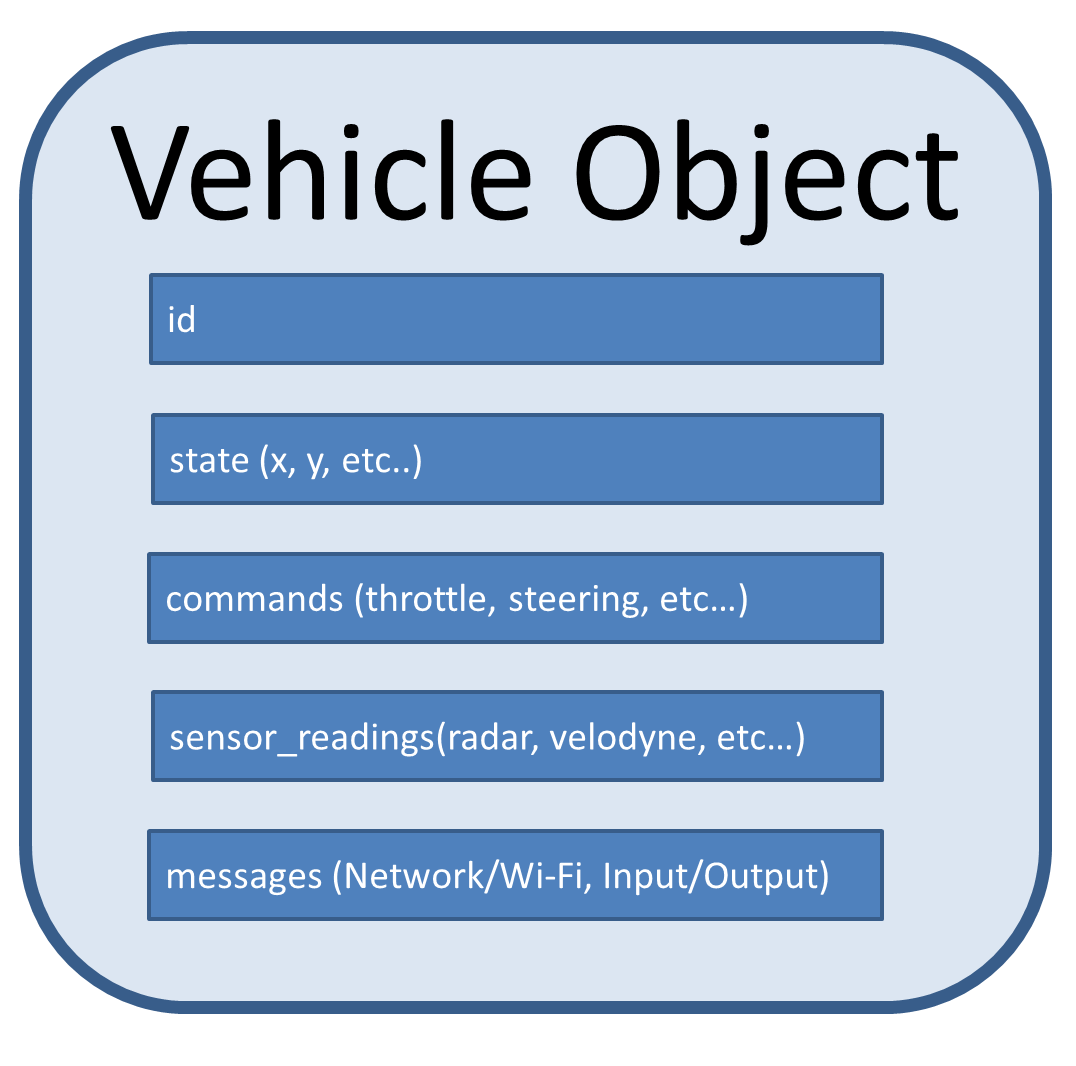
\includegraphics[width=0.6\textwidth]{vehicle_object}
    \caption{Representation of the vehicle object and its basic attributes \label{fig:vehicle_object} }
\end{figure}

\subsection{The SML World Structure}

An explanation of the SML World structure and its fundamental modules will be given here. The explanation will be as simplified as possible, however we will refer to the appropriate sections where these modules are explained in detail.

\subsubsection{The SML World Main Module}

The SML World in its simplest (and most useless form) simply consists of the main module running. This main module is simply used for storing information about vehicles in the world.

A simple depiction of it would be the one shown in figure \ref{fig:sml_world_structure_1}. In this figure, we use the block with name SML World to represent the main module of the SML World. In this module one can see a section of it called Vehicles Dictionary, this is the designation of the memory structure that contains all of the information about current vehicles in the SML World. Implementation wise it is achieved as a Python dictionary, hence the name. The keys of this dictionary are the ids of the vehicles in it. The values of this dictionary will be instances of the Vehicle Class, as explained in \ref{subsec:the_vehicle_structure}.

\begin{figure}[h!]
  \centering
    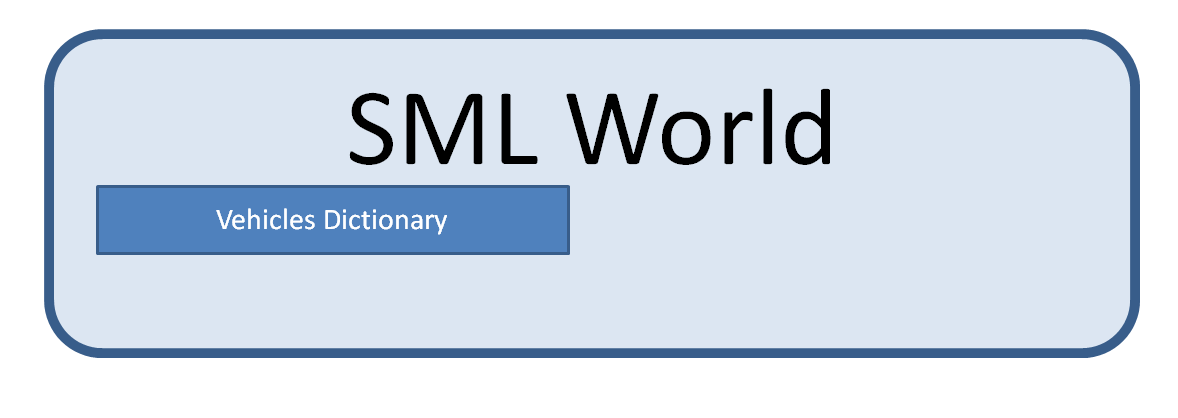
\includegraphics[width=1.0\textwidth]{sml_world_structure_1}
    \caption{The simplest form of the SML World, consisting only in the main module and the Vehicles Dictionary \label{fig:sml_world_structure_1} }
\end{figure}

\subsubsection{The Road Module}

We now add an extra component to our SML World, the Road Module. The Road Module is in charge of the road network, providing functionalities for visualisation and path generation for vehicles. A detailed explanation of it can be found in section \ref{sec:the_road_module}. With the addition of the Road Module the SML World now looks like the structure shown in figure \ref{fig:sml_world_structure_2}.

\begin{figure}[h!]
  \centering
    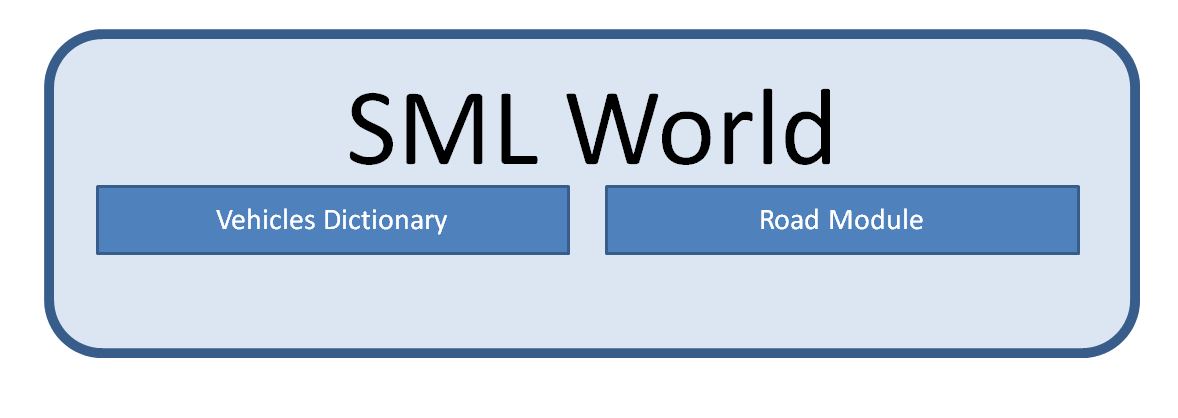
\includegraphics[width=1.0\textwidth]{sml_world_structure_2}
    \caption{The SML World, with the Road Module added \label{fig:sml_world_structure_2} }
\end{figure}

\subsubsection{The Simulation Module}

\label{subsubsec:simulation_module}

In its current state the SML World is able to store information about vehicles and the road network, as implemented by the Vehicles Dictionary and the Road Module. As is now, the SML World will simply be a static environment, as it is simply a container of information. We now add the Simulation Module so that we can get a dynamic world.

The Simulation Module, will be a Python class instantiated by the SML World, that will simulate the vehicles' movements. This class simply accesses the Vehicles Dictionary, and for each vehicle in it, it will perform a state (position, orientation, velocities, etc...) update based on the current state and the current vehicle inputs/commands (throttle, brake, steering, etc...). Besides the state update, the Simulation Module also updates the sensor readings (radar, velodyne, camera inputs, etc...) of each vehicle it simulates.

An important detail of the simulation module is that it is going to be running in parallel, that is, it will have it's own thread of execution. The simulation module will be running at a fixed rate, the higher this rate is, the more accurate the simulation is. A typical value for the simulation rate is somewhere around $50 Hz$.

Figure \ref{fig:sml_world_structure_3} shows the new structure diagram of the SML World with this added module. Notice that in the figure, the Simulation Module not completely contained within the SML World main module. We use this as a symbolic meaning that the Simulation Module is somewhat independent from the SML World, being that it is running on its own thread, but it still relies on it to perform it's task, since it needs to access and change the Vehicles Dictionary.

\begin{figure}[h!]
  \centering
    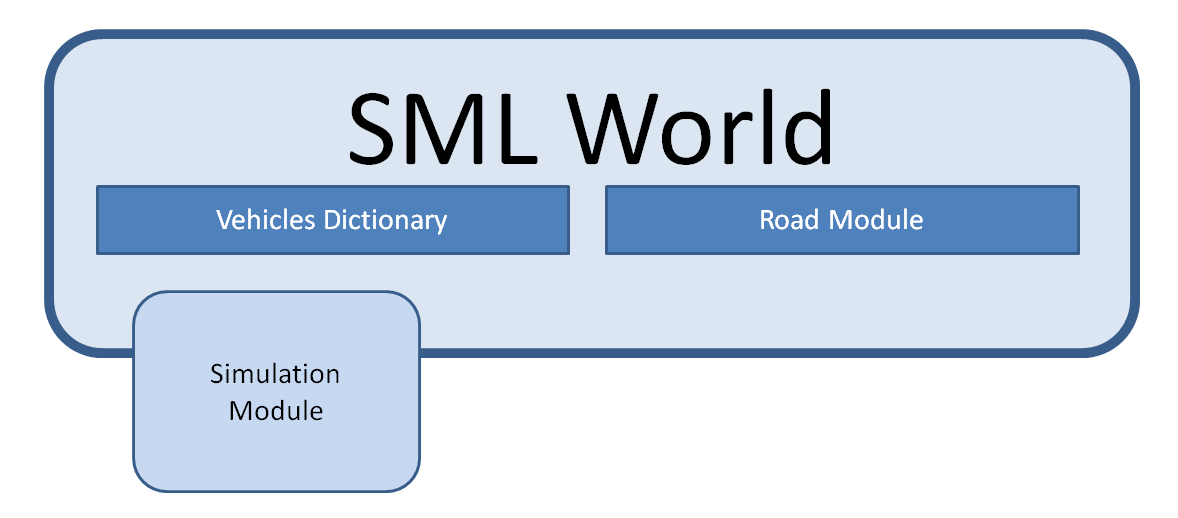
\includegraphics[width=1.0\textwidth]{sml_world_structure_3}
    \caption{The SML World, with a parallel execution thread corresponding to the Simulation Module \label{fig:sml_world_structure_3} }
\end{figure}


With this added module we now have a fully functional driving simulator, as vehicles can be simulated and their states updated according to the throttle and steering commands they have. If the vehicles in the Vehicles Dictionary already implement autonomous driving intelligence, then we can state that we already have a fully functional autonomous driving simulator.

\subsubsection{The V2V Module}

Currently we can achieve autonomous driving with the system as is, however if we wish to go one step further and allow for cooperative autonomous driving we need to provide the Vehicles with communications methods. To do so we use the V2V Module. V2V stands for Vehicle-to-Vehicle communication, and as the name implies it is used to allow vehicles to "talk" with each other.

The V2V Module implements this V2V communication, simulating two possible ways of communication, over the Network or over Wi-Fi. The V2V Module main task will be to make sure that outgoing messages of a vehicle are delivered to the respective vehicles they are destined to. To do so, this module will check the vehicles in the Vehicles Dictionary and update the incoming and outgoing messages that each vehicle has. A detailed explanation can be found in section \ref{sec:the_v2v_module}.

Similarly to the Simulation Module, the V2V Module will run in parallel, in it's own execution thread, at a fixed rate. The updated representation of the SML World structure can be seen in figure \ref{fig:sml_world_structure_4}.

\begin{figure}[h!]
  \centering
    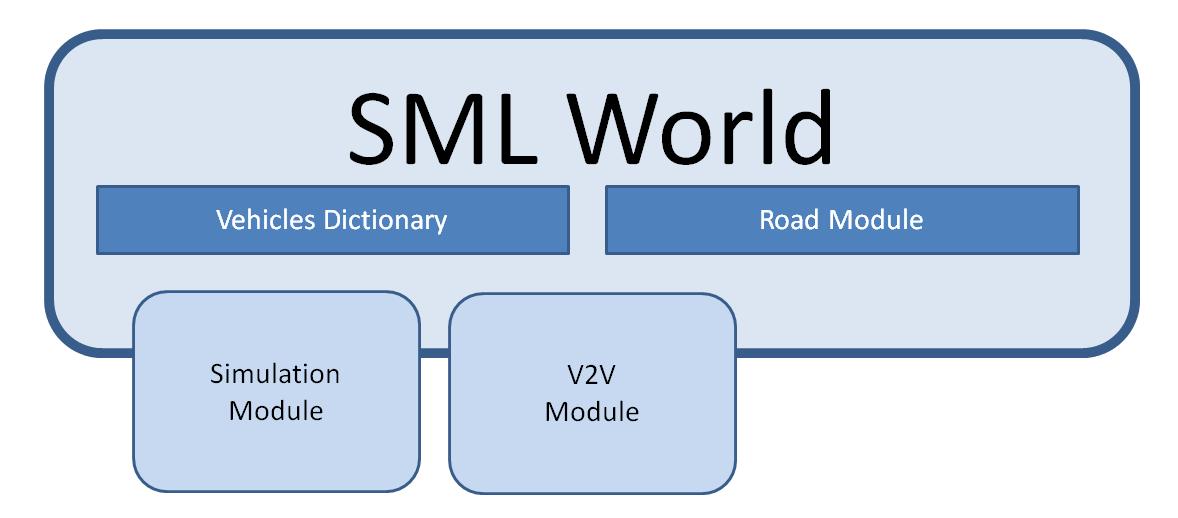
\includegraphics[width=1.0\textwidth]{sml_world_structure_4}
    \caption{The SML World, with a second parallel execution thread corresponding to the V2V Module \label{fig:sml_world_structure_4} }
\end{figure}
